\documentclass[12pt]{article}
\usepackage[utf8]{inputenc}
\usepackage[utf8]{inputenc}
\usepackage{amsmath}
\usepackage{amsthm}
\usepackage{amssymb}
\usepackage{array}
\usepackage{geometry}
\usepackage{amsfonts}
\usepackage{mathrsfs}
\usepackage{bm}
\usepackage{hyperref}
\usepackage{float}
\usepackage[dvipsnames]{xcolor}
\usepackage[inline]{enumitem}
\usepackage{mathtools}
\usepackage{changepage}
\usepackage{graphicx}
\usepackage{systeme}
\usepackage{caption}
\usepackage{subcaption}
\usepackage[linguistics]{forest}
\usepackage{tikz}
\usetikzlibrary{matrix, patterns, decorations.pathreplacing, calligraphy}
\usepackage{tikz-cd}
\usepackage[nameinlink]{cleveref}
\geometry{
headheight=15pt,
left=60pt,
right=60pt
}
\setlength{\emergencystretch}{20pt}
\usepackage{fancyhdr}
\pagestyle{fancy}
\fancyhf{}
\lhead{}
\chead{Section 8.1 Exercises}
\rhead{\thepage}
\hypersetup{
    colorlinks=true,
    linkcolor=blue,
    urlcolor=blue
}

\theoremstyle{definition}
\newtheorem*{remark}{Remark}

\newtheoremstyle{exercise}
    {}
    {}
    {}
    {}
    {\bfseries}
    {.}
    { }
    {\thmname{#1}\thmnumber{#2}\thmnote{ (#3)}}
\theoremstyle{exercise}
\newtheorem{exercise}{Exercise 8.1.}

\newtheoremstyle{solution}
    {}
    {}
    {}
    {}
    {\itshape\color{magenta}}
    {.}
    { }
    {\thmname{#1}\thmnote{ #3}}
\theoremstyle{solution}
\newtheorem*{solution}{Solution}

\Crefformat{exercise}{#2Exercise 8.1.#1#3}

\newcommand{\interior}[1]{%
  {\kern0pt#1}^{\mathrm{o}}%
}
\newcommand{\ts}{\textsuperscript}
\newcommand{\setcomp}[1]{#1^{\mathsf{c}}}
\newcommand{\poly}{\mathcal{P}}
\newcommand{\quand}{\quad \text{and} \quad}
\newcommand{\quimplies}{\quad \implies \quad}
\newcommand{\quiff}{\quad \iff \quad}
\newcommand{\N}{\mathbf{N}}
\newcommand{\Z}{\mathbf{Z}}
\newcommand{\Q}{\mathbf{Q}}
\newcommand{\I}{\mathbf{I}}
\newcommand{\R}{\mathbf{R}}
\newcommand{\C}{\mathbf{C}}

\DeclarePairedDelimiter\abs{\lvert}{\rvert}
% Swap the definition of \abs* and \norm*, so that \abs
% and \norm resizes the size of the brackets, and the 
% starred version does not.
\makeatletter
\let\oldabs\abs
\def\abs{\@ifstar{\oldabs}{\oldabs*}}
%
\let\oldnorm\norm
\def\norm{\@ifstar{\oldnorm}{\oldnorm*}}
\makeatother

\DeclarePairedDelimiter\paren{(}{)}
\makeatletter
\let\oldparen\paren
\def\paren{\@ifstar{\oldparen}{\oldparen*}}
\makeatother

\DeclarePairedDelimiter\bkt{[}{]}
\makeatletter
\let\oldbkt\bkt
\def\bkt{\@ifstar{\oldbkt}{\oldbkt*}}
\makeatother

\DeclarePairedDelimiter\set{\{}{\}}
\makeatletter
\let\oldset\set
\def\set{\@ifstar{\oldset}{\oldset*}}
\makeatother

\setlist[enumerate,1]{label={(\alph*)}}

\begin{document}

\section{Section 8.1 Exercises}

Exercises with solutions from Section 8.1 of \hyperlink{ua}{[UA]}.

\begin{exercise}
\label{ex:1}
    \begin{enumerate}
        \item Explain why both the Riemann sum \( R(f, P) \) and \( \int_a^b f \) fall between \( L(f, P) \) and \( U(f, P) \).

        \item Explain why \( U(f, P') - L(f, P') < \epsilon/3 \).
    \end{enumerate}
\end{exercise}

\begin{solution}
    \begin{enumerate}
        \item The inequality \( L(f, P) \leq R(f, P) \leq U(f, P) \) follows as \( m_k \leq f(c_k) \leq M_k \) for each \( k \) and the inequality \( L(f, P) \leq \int_a^b f \leq U(f, P) \) follows by observing that:
        \begin{itemize}
            \item \( L(f, P) \leq L(f) \);

            \item \( U(f) \leq U(f, P) \);

            \item \( \int_a^b f = L(f) = U(f) \) (as \( f \) is integrable on \( [a, b] \)).
        \end{itemize}

        \item Because \( P' \) is a refinement of \( P \), Lemma 7.2.3 shows that \( U(f, P') - L(f, P') < \epsilon/3 \).
    \end{enumerate}
\end{solution}

\begin{exercise}
\label{ex:2}
    Explain why \( U(f, P) - U(f, P') \geq 0 \).
\end{exercise}

\begin{solution}
    This follows from Lemma 7.2.3, as \( P' \) is a refinement of \( P \).
\end{solution}

\begin{exercise}
\label{ex:3}
    \begin{enumerate}
        \item In terms of \( n \), what is the largest number of terms of the form \( M_k (x_k - x_{k-1}) \) that could appear in one of \( U(f, P) \) or \( U(f, P') \) but not the other?

        \item Finish the proof in this direction by arguing that
        \[
            U(f, P) - U(f, P') < \epsilon/3.
        \]
    \end{enumerate}
\end{exercise}

\begin{solution}
    \begin{enumerate}
        \item Note that
        \[
            \abs{P'} = \abs{P_{\epsilon}} + \abs{P} - \abs{P_{\epsilon} \cap P} = n + 1 + \abs{P} - \abs{P_{\epsilon} \cap P}.
        \]
        To maximize the number of points in \( \abs{P'} \), the above expression shows that \( \abs{P_{\epsilon} \cap P} \) should be minimized. Since both \( P_{\epsilon} \) and \( P \) must contain the points \( a \) and \( b \), the smallest this intersection could be is \( \abs{P_{\epsilon} \cap P} = 2 \) and thus
        \[
            \abs{P'} = n - 1 + \abs{P}
        \]
        is the largest that \( P' \) could be. In other words, after forming \( P' \) by adding new points from \( P_{\epsilon} \) to \( P \), the largest number of points that could have been added is \( n - 1 \). For each of these new points added, two terms are added to \( U(f, P') \) which do not appear in \( U(f, P) \) and there is one term in \( U(f, P) \) which does not appear in \( U(f, P') \); see \Cref{fig:1}.
        \begin{figure}[H]
            \centering
            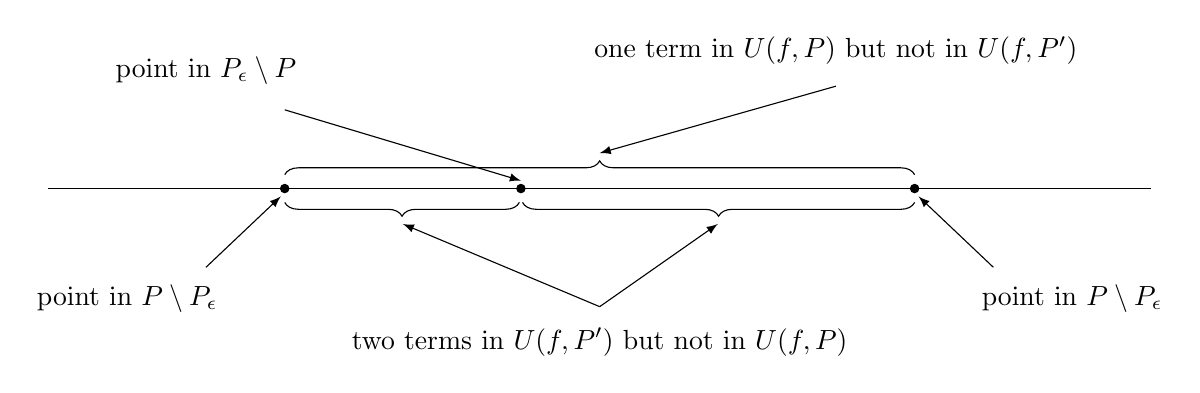
\begin{tikzpicture}
                \draw (-7,0) -- (7,0);

                \filldraw (-4,0) circle (1.5pt);
                \filldraw (-1,0) circle (1.5pt);
                \filldraw (4,0) circle (1.5pt);

                \draw[-latex] (-5,-1) -- (-4.05,-0.1);
                \node at (-6,-1.4) {point in \( P \setminus P_{\epsilon} \)};

                \draw[-latex] (5,-1) -- (4.05,-0.1);
                \node at (6,-1.4) {point in \( P \setminus P_{\epsilon} \)};

                \draw[-latex] (-4,1) -- (-1,0.1);
                \node at (-5,1.5) {point in \( P_{\epsilon} \setminus P \)};

                \draw[decorate, decoration = {brace,mirror,raise=5pt,amplitude=5pt}] (-4,0) -- (-1.02,0);
                \draw[decorate, decoration = {brace,mirror,raise=5pt,amplitude=5pt}] (-0.98,0) -- (4,0);
                \draw[-latex] (0,-1.5) -- (-2.5,-0.45);
                \draw[-latex] (0,-1.5) -- (1.5,-0.45);
                \node at (0,-1.95) {two terms in \( U(f, P') \) but not in \( U(f, P) \)};

                \draw[decorate, decoration = {brace,raise=5pt,amplitude=5pt}] (-4,0) -- (4,0);
                \draw[-latex] (3,1.3) -- (0,0.45);
                \node at (3,1.75) {one term in \( U(f, P) \) but not in \( U(f, P') \)}; 
            \end{tikzpicture}
            \caption{Adding a point to \( P \)}
            \label{fig:1}
        \end{figure}
        It follows that the largest number of terms that could appear in one of \( U(f, P) \) or \( U(f, P') \) but not the other is \( 3(n - 1) \).

        \item Let us write \( U(f, P) - U(f, P') \) as
        \[
            \sum M_k (x_k - x_{k-1}) - \sum M_k (x_k - x_{k-1}),
        \]
        where the sum on the left consists of those terms appearing in \( U(f, P) \) but not in \( U(f, P') \) and the sum on the right consists of those terms appearing in \( U(f, P') \) but not in \( U(f, P) \); terms which appear in both \( U(f, P) \) and \( U(f, P') \) cancel. By part (a), there can be at most \( 3(n - 1) \) terms in total across both sums. \Cref{ex:2} shows that the quantity \( U(f, P) - U(f, P') \) is non-negative and thus
        \begin{multline*}
            U(f, P) - U(f, P') = \abs{U(f, P) - U(f, P')} = \abs{\sum M_k (x_k - x_{k-1}) - \sum M_k (x_k - x_{k-1})} \\[2mm]
            \leq \sum \abs{M_k} (x_k - x_{k-1}) + \sum \abs{M_k} (x_k - x_{k-1}).
        \end{multline*}
        Now we can use the fact that both partitions \( P \) and \( P' \) are \( \delta \)-fine, that \( M \) is a bound on \( \abs{f} \), and that there are at most \( 3(n - 1) \) terms in total across both sums to see that
        \[
            U(f, P) - U(f, P') \leq 3(n - 1) M \delta < \frac{\epsilon}{3}.
        \]
    \end{enumerate}
\end{solution}

\begin{exercise}
\label{ex:4}
    \begin{enumerate}
        \item Show that if \( f \) is continuous, then it is possible to pick tags \( \{ c_k \}_{k=1}^n \) so that
        \[
            R(f, P) = U(f, P).
        \]
        Similarly, there are tags for which \( R(f, P) = L(f, P) \) as well.

        \item If \( f \) is not continuous, it may not be possible to find tags for which \( R(f, P) = U(f, P) \). Show, however, that given an arbitrary \( \epsilon > 0 \), it is possible to pick tags for \( P \) so that
        \[
            U(f, P) - R(f, P) < \epsilon.
        \]
        The analogous statement holds for lower sums.
    \end{enumerate}
\end{exercise}

\begin{solution}
    \begin{enumerate}
        \item For \( k \in \{ 1, \ldots, n \} \), the Extreme Value Theorem (Theorem 4.4.2) implies that \( f \) attains its maximum on the compact set \( [x_{k-1}, x_k] \), i.e.\ there is some \( c_k \in [x_{k-1}, x_k] \) such that \( f(c_k) = M_k \). Thus choosing the collection of tags \( \{ c_k \}_{k=1}^n \) gives us \( R(f, P) = U(f, P) \). Similarly, the Extreme Value Theorem implies that \( f \) attains its minimum on \( [x_{k-1}, x_k] \) at some \( c_k \in [x_{k-1}, x_k] \); choosing the tags \( \{ c_k \}_{k=1}^n \) gives us \( R(f, P) = L(f, P) \).

        \item Suppose \( P = \{ x_0, \ldots, x_n \} \). By Lemma 1.3.8, for each \( k \in \{ 1, \ldots, n \} \), there exists some \( c_k \in [x_{k-1}, x_k] \) such that
        \[
            M_k - \frac{\epsilon}{b - a} < f(c_k) \leq M_k.
        \]
        Choose the tags \( \{ c_k \}_{k=1}^n \) and then observe that
        \[
            U(f, P) - R(f, P) = \sum_{k=1}^n (M_k - f(c_k)) \Delta x_k < \frac{\epsilon}{b - a} \sum_{k=1}^n \Delta x_k = \epsilon.
        \]
        The analogous statement for lower sums can be proved similarly.
    \end{enumerate}
\end{solution}

\begin{exercise}
\label{ex:5}
    Use the results of the previous exercise to finish the proof of Theorem 8.1.2.
\end{exercise}

\begin{solution}
    See \href{https://lew98.github.io/Mathematics/UA_Section_7_2_Exercises.pdf}{Exercise 7.2.6}.
\end{solution}

\begin{exercise}
\label{ex:6}
    Consider the interval \( [0, 1] \).
    \begin{enumerate}
        \item If \( \delta(x) = 1/9 \), find a \( \delta(x) \)-fine tagged partition of \( [0, 1] \). Does the choice of tags matter in this case?

        \item Let
        \[
            \delta(x) = \begin{cases}
                1/4 & \text{if } x = 0 \\
                x/3 & \text{if } 0 < x \leq 1.
            \end{cases}
        \]
        Construct a \( \delta(x) \)-fine tagged partition of \( [0, 1] \).
    \end{enumerate}
\end{exercise}

\begin{solution}
    \begin{enumerate}
        \item Take \( P = \set{ 0, \tfrac{1}{10}, \tfrac{2}{10}, \ldots, \tfrac{9}{10}, 1 } \) and for each \( k \in \{ 1, \ldots, 10 \} \) choose the tag \( c_k = \frac{k}{10} \). Then
        \[
            \Delta x_k = \frac{1}{10} < \frac{1}{9} = \delta(c_k).
        \]
        The choice of tags is irrelevant here since the gauge \( \delta \) is constant.

        \item Let \( P = \set{ 0, \tfrac{3}{15}, \tfrac{4}{15}, \tfrac{5}{15}, \ldots, \tfrac{14}{15}, 1 } \) and choose the tags \( c_1 = 0 \) and \( c_k = \tfrac{k + 2}{15} \) for \( 2 \leq k \leq 13 \). Some tedious calculations show that this tagged partition is \( \delta(x) \)-fine.
    \end{enumerate}
\end{solution}

\begin{exercise}
\label{ex:7}
    Finish the proof of Theorem 8.1.5.
\end{exercise}

\begin{solution}
    Denote the two halves by
    \[
        J_1 = \bkt{ a, \frac{a + b}{2} } \quand J_2 = \bkt{ \frac{a + b}{2}, b }.
    \]
    If there exists a \( c_1 \in J_1 \) and a \( c_2 \in J_2 \) such that \( \tfrac{b - a}{2} < \delta(c_1) \) and \( \tfrac{b - a}{2} < \delta(c_2) \), then the tagged partition
    \[
        \paren{ P = \set{ a, \frac{a + b}{2}, b }, \{ c_1, c_2 \} }
    \]
    is \( \delta(x) \)-fine. Otherwise, at least one of the following statements is true:
    \begin{itemize}
        \item for all \( x \in J_1, \delta(x) \leq \tfrac{b - a}{2} \);

        \item for all \( x \in J_2, \delta(x) \leq  \tfrac{b - a}{2} \).
    \end{itemize}
    For each of the intervals for which the relevant statement above is true, we perform the same procedure: bisect the interval into two equal halves and look for valid tags. By continuing this algorithm, we form a ``tree'' as in \Cref{fig:2}.

    \begin{figure}[H]
        \centering
        \scalebox{1.0}{
            \begin{forest}
                for tree={s sep=10mm}
                [{$[a, b]$}, nice empty nodes
                    [
                        [F]
                        [
                            [F]
                            [F]
                        ]
                    ]
                    [
                        [F]
                        [
                            [
                                [F]
                                [F]
                            ]
                            [F]
                        ]
                    ]
                ]
            \end{forest}
        }
        \caption{Found a \( \delta(x) \)-fine tagged partition}
        \label{fig:2}
    \end{figure}
    
    Each node (other than the topmost) of the tree represents a closed and bounded interval which is exactly half of its parent node: the left half if the node is to the left of its parent and the right half if the node is to the right of its parent; note that the length of each node is exactly half of the length of its parent node. An ``F'' indicates that we found a valid tag at that node, i.e.\ if the node is an interval \( J \), then we found some \( c \in J \) such that \( \abs{J} < \delta(c) \).

    If this algorithm stops after a finite number of steps, i.e.\ if the tree is finite as in \Cref{fig:2}, then we may take the collection of endpoints of the terminal nodes and the tags we found there as our \( \delta(x) \)-fine tagged partition. The alternative is that the algorithm does not terminate after a finite number of steps, as in \Cref{fig:3}.

    \begin{figure}[H]
        \centering
        \scalebox{1.0}{
            \begin{forest}
                for tree={s sep=10mm}
                [\textcolor{red}{$I_0 = [a, b]$}, nice empty nodes
                    [
                        [F]
                        [
                            [F]
                            [F]
                        ]
                    ]
                    [\textcolor{red}{$I_1$},edge=red
                        [F]
                        [\textcolor{red}{$I_2$},edge=red
                            [\textcolor{red}{$I_3$},edge=red
                                [\textcolor{red}{$I_4$},edge=red
                                    [F]
                                    [$\vdots$,edge=red]
                                ]
                                [F]
                            ]
                            [F]
                        ]
                    ]
                ]
            \end{forest}
        }
        \caption{Algorithm does not terminate}
        \label{fig:3}
    \end{figure}
    
    We will show that this cannot happen. Indeed, if the algorithm fails to terminate, then we obtain a nested sequence of closed and bounded intervals \( (I_n) \) (by following the branches of the tree downwards, e.g.\ the red path in \Cref{fig:3}; there may be more than one such path) such that:
    \begin{enumerate}[label=(\roman*)]
        \item \( \abs{I_n} = \tfrac{b - a}{2^n} \to 0 \);

        \item for all \( x \in I_n \) we have \( \delta(x) \leq \abs{I_n} \).
    \end{enumerate}
    The Nested Interval Property (Theorem 1.4.1) implies that there exists some \( x_0 \in \bigcap_{n=1}^{\infty} I_n \). Property (ii) then implies that \( \delta(x_0) \leq \abs{I_n} \) for all \( n \in \N \); together with property (i), this means that \( \delta(x_0) \leq 0 \), contradicting that \( \delta \) is a gauge. Hence it must be the case that the algorithm stops after a finite number of steps, yielding a \( \delta(x) \)-fine tagged partition.
\end{solution}

\begin{exercise}
\label{ex:8}
    Finish the argument.
\end{exercise}

\begin{solution}
    Let \( \epsilon > 0 \) be given. Because \( f \) has generalized Riemann integrals \( A_1 \) and \( A_2 \), there exist gauges \( \delta_1 \) and \( \delta_2 \) on \( [a, b] \) such that:
    \begin{enumerate}[label=(\roman*)]
        \item for each tagged partition \( \paren{ P, \{ c_k \}_{k=1}^n } \) that is \( \delta_1 \)-fine, the inequality \( \abs{R(f, P) - A_1} < \tfrac{\epsilon}{2} \) holds;

        \item for each tagged partition \( \paren{ P, \{ c_k \}_{k=1}^n } \) that is \( \delta_2 \)-fine, the inequality \( \abs{R(f, P) - A_2} < \tfrac{\epsilon}{2} \) holds.
    \end{enumerate}
    Let \( \delta : [a, b] \to \R \) be the gauge on \( [a, b] \) given by \( \delta(x) = \min \{ \delta_1(x), \delta_2(x) \} \). By Theorem 8.1.5, there exists a tagged partition \( \paren{ P, \{ c_k \}_{k=1}^n } \) that is \( \delta \)-fine; it is straightforward to verify that this tagged partition is also \( \delta_1 \)- and \( \delta_2 \)-fine. It then follows from (i) and (ii) that
    \[
        \abs{A_1 - A_2} \leq \abs{R(f, P) - A_1} + \abs{R(f, P) - A_2} < \epsilon.
    \]
    Since \( \epsilon > 0 \) was arbitrary, we may conclude that \( A_1 = A_2 \).
\end{solution}

\begin{exercise}
\label{ex:9}
    Explain why every function that is Riemann-integrable with \( \int_a^b f = A \) must also have generalized Riemann integral \( A \).
\end{exercise}

\begin{solution}
    For any \( \epsilon > 0 \), we can simply take the gauge on \( [a, b] \) to be the constant function whose value is the \( \delta \) supplied by Theorem 8.1.2.
\end{solution}

\begin{exercise}
\label{ex:10}
    Show that if \( \paren{ P, \{ c_k \}_{k=1}^n } \) is a \( \delta(x) \)-fine tagged partition, then \( R(g, P) < \epsilon \).
\end{exercise}

\begin{solution}
    Suppose \( P = \{ x_0, \ldots, x_n \} \). If each \( c_k \) is irrational then \( R(g, P) = 0 < \epsilon \); otherwise, let \( \{ c_{k_1}, \ldots, c_{k_m} \} \) be the collection of rational tags, so that for each \( 1 \leq j \leq m \), we have \( c_{k_j} = r_{i_j} \) for some (not necessarily unique) \( i_j \). It follows that
    \[
        R(g, P) = \sum_{k=1}^n g(c_k) \Delta x_k = \sum_{j=1}^m \Delta x_{k_j} < \sum_{j=1}^m \delta \paren{ c_{k_j} } = \sum_{j=1}^m \delta \paren{ r_{i_j} } = \sum_{j=1}^m \frac{\epsilon}{2^{i_j + 1}}.
    \]
    Since a tag can appear in at most two subintervals, any given rational number \( r_i \) can appear at most twice in the collection \( \{ r_{i_1}, \ldots, r_{i_m} \} \). Thus
    \[
        R(g, P) < \sum_{j=1}^m \frac{\epsilon}{2^{i_j + 1}} \leq 2 \sum_{i=1}^{\infty} \frac{\epsilon}{2^{i + 1}} = \epsilon.
    \]
\end{solution}

\begin{exercise}
\label{ex:11}
    Show that
    \[
        F(b) - F(a) = \sum_{k=1}^n [F(x_k) - F(x_{k-1})].
    \]
\end{exercise}

\begin{solution}
    This is a telescoping sum:
    \[
        \sum_{k=1}^n [F(x_k) - F(x_{k-1})] = F(x_n) - F(x_0) = F(b) - F(a).
    \]
\end{solution}

\begin{exercise}
\label{ex:12}
    For each \( c \in [a, b] \), explain why there exists a \( \delta(c) > 0 \) (a \( \delta > 0 \) depending on \( c \)) such that
    \[
        \abs{\frac{F(x) - F(c)}{x - c} - f(c)} < \epsilon
    \]
    for all \( 0 < \abs{x - c} < \delta(c) \).
\end{exercise}

\begin{solution}
    By assumption the function \( F \) is differentiable at \( c \) and satisfies \( F'(c) = f(c) \); the existence of such a \( \delta(c) \) is then immediate from the definition of \( F'(c) \) as
    \[
        \lim_{x \to c} \frac{F(x) - F(c)}{x - c}.
    \]
\end{solution}

\begin{exercise}
\label{ex:13}
    \begin{enumerate}
        \item For a particular \( c_k \in [x_{k-1}, x_k] \) of \( P \), show that
        \[
            \abs{F(x_k) - F(c_k) - f(c_k)(x_k - c_k)} < \epsilon (x_k - c_k)
        \]
        and
        \[
            \abs{F(c_k) - F(x_{k-1}) - f(c_k)(c_k - x_{k-1})} < \epsilon (c_k - x_{k-1}).
        \]

        \item Now, argue that
        \[
            \abs{F(x_k) - F(x_{k-1}) - f(c_k)(x_k - x_{k-1})} < \epsilon (x_k - x_{k-1}),  
        \]
        and use this fact to complete the proof of the theorem.
    \end{enumerate}
\end{exercise}

\begin{solution}
    \begin{enumerate}
        \item The inequalities here should not be strict; the first strict inequality fails if \( c_k = x_k \) and the second fails if \( c_k = x_{k-1} \). Instead, we'll show that
        \[
            \abs{F(x_k) - F(c_k) - f(c_k)(x_k - c_k)} \leq \epsilon (x_k - c_k)
        \]
        and
        \[
            \abs{F(c_k) - F(x_{k-1}) - f(c_k)(c_k - x_{k-1})} \leq \epsilon (c_k - x_{k-1}),
        \]
        which is sufficient for the proof. For the first inequality, note that both sides are zero if \( c_k = x_k \). Suppose therefore that \( x_{k-1} \leq c_k < x_k \) and note that, because the tagged partition \( (P, \{ c_k \}) \) is \( \delta \)-fine, we have \( 0 < x_k - c_k \leq \Delta x_k < \delta(c_k) \). It follows from \Cref{ex:12} that
        \[
            \abs{\frac{F(x_k) - F(c_k)}{x_k - c_k} - f(c_k)} < \epsilon.
        \]
        Multiplying through by \( x_k - c_k \), which is positive, gives the desired inequality; the second inequality is obtained similarly.

        \item Expressing the inequalities from part (a) as
        \begin{gather*}
            -\epsilon (x_k - c_k) \leq F(x_k) - F(c_k) - f(c_k)(x_k - c_k) \leq \epsilon (x_k - c_k) \\[2mm]
            -\epsilon (c_k - x_{k-1}) \leq F(c_k) - F(x_{k-1}) - f(c_k)(c_k - x_{k-1}) \leq \epsilon (c_k - x_{k-1})
        \end{gather*}
        and adding the rows together, we see that
        \[
            -\epsilon(x_k - x_{k-1}) \leq F(x_k) - F(x_{k-1}) - f(c_k)(x_k - x_{k-1}) \leq \epsilon(x_k - x_{k-1}).
        \]
        Thus
        \begin{multline*}
            \abs{F(b) - F(a) - R(f, P)} \leq \sum_{k=1}^n \abs{F(x_k) - F(x_{k-1}) - f(c_k)(x_k - x_{k-1})} \\
            \leq \sum_{k=1}^n \epsilon (x_k - x_{k-1}) \leq \epsilon (b - a).
        \end{multline*}
        By replacing \( \epsilon \) in the proof with \( \tfrac{\epsilon}{2(b - a)} \), we obtain
        \[
            \abs{F(b) - F(a) - R(f, P)} < \epsilon,
        \]
        as desired.
    \end{enumerate}
\end{solution}

\begin{exercise}
\label{ex:14}
    \begin{enumerate}
        \item Why are we sure that \( f \) and \( (F \circ g)' \) have generalized Riemann integrals?

        \item Use Theorem 8.1.9 to finish the proof.
    \end{enumerate}
\end{exercise}

\begin{solution}
    \begin{enumerate}
        \item Both \( f = F' \) and \( (F \circ g)' \) are derivatives; Theorem 8.1.9 implies that any derivative is generalized-Riemann-integrable.

        \item By the chain rule and Theorem 8.1.9:
        \[
            \int_a^b (f \circ g) \cdot g' = \int_a^b (F' \circ g) \cdot g' = \int_a^b (F \circ g)' = F(g(b)) - F(g(a)) = \int_{g(a)}^{g(b)} F' = \int_{g(a)}^{g(b)} f.
        \]
    \end{enumerate}
\end{solution}

\noindent \hrulefill

\noindent \hypertarget{ua}{\textcolor{blue}{[UA]} Abbott, S. (2015) \textit{Understanding Analysis.} 2\ts{nd} edition.}

\end{document}